
\begin{opin}{\guscolor}{Gustavo}

\end{opin}

\begin{opin}{\victorcolor}{Víctor}

No pude asistir a esa clase.

\end{opin}

\begin{opin}{\pedrocolor}{Pedro}

El empleo por parte del profesor de ciertos recursos didácticos, puede llegar a cubrir en cierta media las carencias de los alumnos que presentan algún tipo de dificultad. Esta actitud, es el pilar fundamental para lograr que el concepto de educación inclusiva sea real dentro del aula.

Como bien ha dicho Raquel, para poder comprender mejor como atender estas NEE (Necesidades Especiales Educativas) es necesario tener contacto con todos los recurso educativos existente en la red.  Por eso resulta necesario hablar de:

\begin{itemize}
\item \textbf{ Proyecto Aprender  :} Se presenta como un Recurso Multimedia Interactivo que tiene como principal objetivo afianzar y desarrollar las capacidades físicas, afectivas, cognitivas y comunicativas de los alumnos con necesidades educativas. Para lograr este fin, promueve la utilización de Nuevas Tecnologías de la Información y Comunicación.

\item \textbf{Creena (Gobierno de Navarra):} Podemos encontrar documentación sobre diferentes trastornos de comportamiento, libros, enlaces, recursos educativos especiales, etc.

\begin{minipage}[h]{1.0\linewidth}
\centering
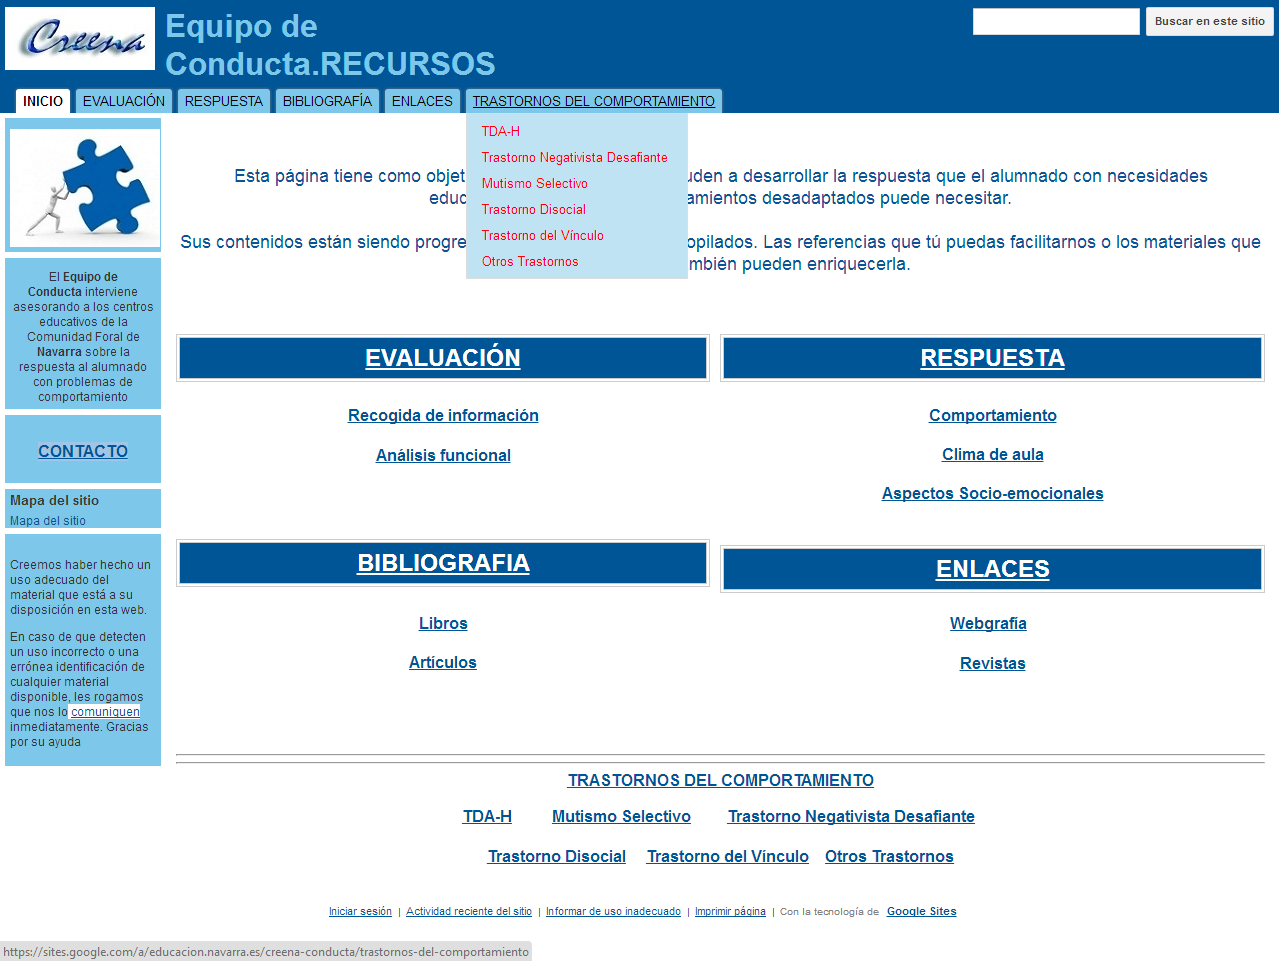
\includegraphics[scale=0.3]{img/tdah_pedro1.png}
%\captionof{figure}{Esquema de la posición de la amígdala en el cerebro humano.}
\end{minipage}

\item \textbf{Cedec:}  Realiza un estudio pormenorizado de los diferentes tipos de discapacidades, respondiendo a preguntas como: ¿Qué es? ¿Cuáles son las causas? ¿Cómo se detecta? ¿Qué hacer y cómo actuar? Además podemos encontrar varios libros publicados con posibilidad de descarga.
\end{itemize}

Una vez vistos los recursos que podemos encontrar en la web, nos centramos en dos trastornos de aprendizaje específico; La Discalculia y El Trastorno por Déficit de Atención con o sin Hiperactividad TDAH.

\subsubsection{Discalculia}
\index{Discalculia}

\begin{itemize}
\item \textbf{¿Dificultad de aprendizaje que conlleva?}
\begin{itemize}
\item Dificultad de comprender y realizar cálculos matemáticos
\item Dificultad en efectuar una buena coordinación espacial y temporal.
\item Dificultad a la hora de recordar conceptos o los pasos para resolver varios cálculos.
\item Dificultades para operaciones cotidianas sencillas, con monedas o números 	
\end{itemize}

\item \textbf{¿Cuáles son criterios de diagnóstico?}
\begin{itemize}
\item DSM-V. Manual Diagnóstico y Estadístico de los Trastorno Mentales.
\end{itemize}

\item \textbf{¿En qué aéreas se presenta esta deficiencia?}
\begin{itemize}
\item \textit{Destreza lingüística :} Deficiencias en la comprensión de términos matemáticos y la conversión de problemas matemáticos en símbolos matemáticos.
\item \textit{Destreza de percepción :} Dificultad en la capacidad para reconocer y entender los símbolos. También para ordenar grupos de números.
\item \textit{Destreza matemática :} Se incluye la dificultad con las operaciones básicas y sus secuencias (suma, resta, multiplicación y división).
\item \textit{Destreza de atención:} Se trata de dificultades en copiar figuras y observar los símbolos operacionales correctamente.
\end{itemize}

\item \textbf{¿Cómo podemos ayudar a estos alumnos?}
\begin{itemize}
\item No poner nervioso al alumno, y darle el tiempo suficiente para que  visualicen y enciendan el problema.
\item Llevar los problemas matemáticos a la vida real. Una enseñanza más práctica.
\item Motivación del alumno, explicándole que con esfuerzo y paciencia logrará los objetivos.
\item Adaptar la evaluación a las características de estos niños.
\item Realizar la resolución del problema paso a paso.

\end{itemize}
\end{itemize}

\subsubsection{Trastorno por Déficit de Atención con o sin Hiperactividad (TDAH):}
\index{TDAH}

\begin{itemize}

\item \textbf{¿Qué síntomas presenta?}
\begin{itemize}
\item Se distrae con estímulos irrelevantes.
\item Descuidado en tareas diarias.
\item Mueve en exceso las manos o pies, remueve en el asiento.
\item Corre, salta excesivamente en situaciones inapropiadas.
\item Habla en exceso
\item Dificultad para guardar turno.
\item Abandona su asiento en clase.
\item Empieza proyectos sin leer o ni escuchar las indicaciones.
\end{itemize}

\item \textbf{¿Cuáles son criterios de diagnóstico?}
\begin{itemize}
\item DSM-V. Manual Diagnóstico y Estadístico de los Trastorno Mentales. Incluye el diagnóstico de TDAH en adultos.
\end{itemize}

\item \textbf{¿Cómo podemos ayudar a estos alumnos?}
\begin{itemize}
\item Recompensando la conducta de poner atención.
\item Enseñar estrategias de resolución de problemas.
\item Que expongan ante los demás los resultados de su trabajo.
\item Actuar, más que hablar.
\item Prever las probables dificultades y establecer un plan para superarlas.
\item Reducir la cantidad total de trabajo.
\item Colocar al alumno cerca del profesor.
\item Información a los padres de la evolución del alumno.
\item Empleo de metodologías activas en el aula.
\item Proporcionar ayuda después del tiempo de clase.
\end{itemize}
\end{itemize}


\end{opin}

\begin{opin}{\virgicolor}{Virginia}

Considero que es vital para mejorar el aprendizaje cambiar el método tradicional de clase magistral por otras metodologías en las que el alumno trabaje de forma activa y colaborativa con los compañeros, se empleen más recursos tecnológicos y se haga uso de las matemáticas recreativas y manipulativas. Todo esto creo que adquiere mayor relevancia si hablamos de alumnos con problemas de aprendizaje ya que:

\begin{itemize}
\item Les ayuda a desarrollar tareas que de otra forma no podrían o sería más difícil.
\item Se compensan las limitaciones propias de su discapacidad.
\item Si se usa de forma efectiva se puede garantizar la igualdad de oportunidades.
\end{itemize}

Muy interesante en este punto el Proyecto Aprender, Proyecto de Necesidades Educativas Especiales. Estos niños tienen unas necesidades educativas especiales por lo que van a precisar determinadas ayudas pedagógicas para el logro de sus fines educativos.  Para el alumnado me parecen muy atractiva las animaciones: 

\url{http://recursostic.educacion.es/aeduc/aprender/web/generales/marco.swf}

También he visto mucha información sobre diferentes trastornos de conducta, así como síndrome de Asperger, TDAH… en el siguiente blog:

\url{http://entrepasillosyaulas.blogspot.com.es/p/profesorado.html}

\subsubsection{Discalculia}

La discalculia es la versión numérica de la dislexia y es reconocida como enfermedad por el DSMIV y por la SOCIEDAD MÉDICA (Clasificación internacional de enfermedades). No existen problemas mentales asociados por lo que no hay problemas en otras áreas que no sea en las que conllevan números o conceptos abstractos de tiempo, direcciones u operaciones de cálculo. Me parece muy importante las pistas que nos llevarían a pensar que un niño tiene discalculia, algunas de ellas son:

\begin{itemize}
\item Uso de los dedos en las operaciones más simples.

\item Problemas con la orientación. 

\item Dificultad en las operaciones y problemas sencillos.

\item Problemas al interpretar enunciados de problemas.

\item Dificultad en su capacidad de memorizar series de números.

\item En los niños mayores de secundaria está afectado el razonamiento.
\end{itemize}

Este problema se puede corregir y para ello hay que reeducar a este tipo de alumnos. Así, la labor del profesor tiene que ser entre otras la de motivarles y hacerles ver que son capaces, al igual que lo son en otras asignaturas.  Es importante para su reeducación que no haya limitaciones de tiempo en las tareas a realizar, que se empleen recursos informáticos y que se adapte la evaluación a las características de estos niños.

En la web: \url{http://www.discalculia.es/discalculia/el_tratamiento.html}, se recomienda el uso del método NUMMERUS (\url{http://www.nummerus.com}) para fortalecer el concepto numérico básico, la utilización de los números empleando actividades de juego, y el uso de una aproximación multisensorial.

Interesante el apartado “para saber más“ de la siguiente página web:

\url{http://procomun.educalab.es/es/ode/view/1418174774696}

\subsubsection{TDAH}

El TDAH es un trastorno de origen neurobiológico, cuyos síntomas provocan en el niño las siguientes conductas:

\begin{itemize}
\item Hiperactividad: presenta un nivel superior e inapropiado de actividad para su edad.

\item Impulsividad: le cuesta controlar sus conductas, emociones y pensamientos.

\item Inatención: tiene una gran dificultad para prestar atención y concentrarse.
\end{itemize}
De nuevo me parece de vital importancia conocer algunas conductas típicas para poder detectarlo de forma temprana:
\begin{itemize}
\item No pueden parar quietos.

\item Se distraen con facilidad.

\item Suelen perder u olvidar cosas y son muy desorganizados en sus trabajos.

\item Actúan sin reflexionar.

\item Pueden pasar horas con la consola, pero son incapaces de atender en clase, por lo que suele ser una de las causas frecuentes de bajo rendimiento académico y dificultades de aprendizaje.

\item Suelen tener problemas en sus relaciones sociales.
\end{itemize}
Muy claro el video donde resumen que es, a quien le afecta, síntomas, subtipos y condiciones para asociarlos: \url{https://www.youtube.com/watch?v=hV7yd11trbk} y muy completas la webs: 

\begin{itemize}
\item \url{http://www.fundacioncadah.org/web/.} Para nosotros como futuros docentes de especial interés es el apartado de docencia y formación para poder asistir a charlas y realizar cursos.

\item \url{http://procomun.educalab.es/es/ode/view/1417742812778} 
\end{itemize}

Como curiosidad \textit{“la creatividad y originalidad que suele caracterizar a las personas con TDAH permite una casi interminable galería de personas famosas y exitosas”}, entre ellos Albert Einstein:  

\url{http://www.sld.cu/galerias/pdf/sitios/rehabilitacion-arte/galeria_de_famosos_con_tdah.pdf}

De nuevo la labor del profesor es fundamental para que estos alumnos trabajen mejor, les ayudemos a subir su autoestima, se sientan integrados, etc. En la web \url{http://www.tdahytu.es/manejar-el-tdah-en-clase/} , nos dan unas pautas de cómo manejar este problema en el aula creando tres ambientes:

\begin{itemize}
\item Ambiente estructurado.

\item Ambiente predecible.

\item Ambiente adecuado para el aprendizaje.
\end{itemize}
\subsubsection{Inteligencias múltiples}

Como se describe en la web: \url{http://www.fundacioncadah.org/web/articulo/la-importancia-de-la-teoria-de-las-inteligencias-multiples-en-el-tdah.html}, la Teoría de las Inteligencias Múltiples (IM) es un modelo de funcionamiento cognitivo propuesto en el año 1983 por Howard Gardner que postula que la inteligencia agrupa diferentes capacidades específicas, esto es, un conjunto de inteligencias múltiples, distintas, diferenciadas entre sí e independientes pero interrelacionadas (ver figura \ref{img:intmult}) 


\begin{minipage}[h]{1.0\linewidth}
\centering
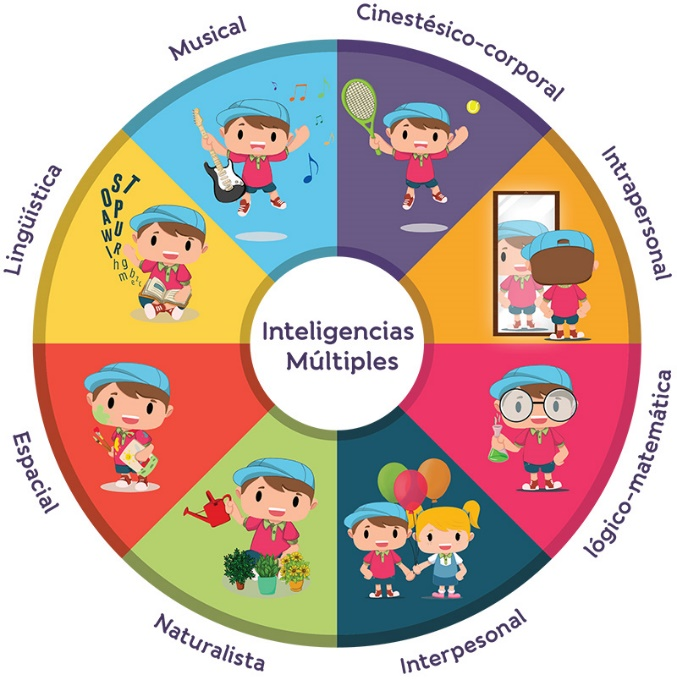
\includegraphics[scale=0.8]{img/im.jpg}
\captionof{figure}{Inteligencias múltiples.}
\label{img:intmult}
\end{minipage}



Creo que es importante conocer cuales de estas habilidades tienen más desarrollada los alumnos para poder perfeccionar los métodos de aprendizaje en función de dichas habilidades sobresalientes.


\end{opin}


